
% !TEX root = ../main.tex

% Local Variables:
% TeX-master: "../main"
% End:
% chktex-file 26

%%%%%%%%%%%%%%%%%%%%%%%%%%%%%%% Header %%%%%%%%%%%%%%%%%%%%%%%%%%%%%%%%%%%%%%%%%%%%
\begin{minipage}[l]{0.42\textwidth}
    \includegraphics[width=1\textwidth]{img/logo-UNAMBA.png}
\end{minipage}
\hfill
\begin{minipage}[c]{0.5\textwidth}
    \begin{flushright}
	\large{\textbf{Unidad \#2}}\\
	\large{Lectures on Física I}\\
	\large{02 de Septiembre del 2025. Haquira, Apurimac}\\
        % \large{\textbf{Student:} Huallpa Aimituma Josué David}
    \end{flushright}
\end{minipage}
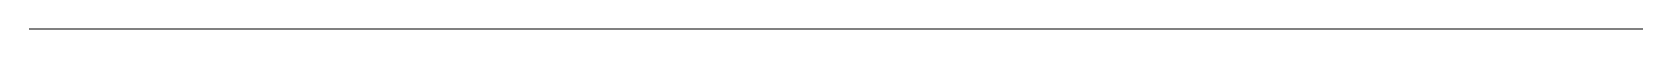
\begin{tikzpicture}
    \draw[gray,thick] (-6.5,0)--(14,0);
\end{tikzpicture}


 %%%%%%%%%%%%%%%%%%%%%%%% INICIO DEL CONTENIDO EN DOS COLUMNAS %%%%%%%%%%%%%%%%%%%%%

 \begin{multicols}{2}
     \begin{center}
         \LARGE{\textbf{Capítulo IV: Cinemática del punto}}\\	
         \vspace{0.2cm}
         % \Large {Lecturers Esteban Chalbaud \& Daniel Galviz} \\
         % \large{Teaching Assistant: Mauricio Gamonal \& Irvin Martínez}\\
         % \large{PhysicsLatam.com}\\
         % \vspace{0.2cm}
         \large{Fecha de entrega: 02 Septiembre 2025, 5:59 pm (GMT-4)}\\
         % \vspace{0.2cm}
         \large{— Evaluación Sust. Unidad III —}
     \end{center}
    
    %%%%%%%%%%%%%%%%%%%%%%%%%%%%%excercise%%%%%%%%%%%%%%%%%%%%%%%%%%%%%%%%%%%%%%%%
    % \begin{excercise}[][][]{ex:k0}{
    %    \textbf{(3 pts.)} Una partícula se mueve en el plano $xy$ con aceleración constante.        
    %    \begin{equation*}
    %        \vec{a}=6\vec{\imath}+4\vec{\jmat}
    %    \end{equation*}
    %    En el instante $t=0$, la velocidad es cero, y el vector posición esta dado por:
    %    \begin{equation*}
    %        \vec{r}=10\vec{\imath}
    %    \end{equation*}
    %    \begin{itemize}
    %        \item[a)] Hallar el vector velocidad y vector posición de la particula en un instante cualquiera $t$.
    %        \item[b)] Elimine el tiempo y obtenga la ecuación cartesiana de la trayectoria en el plano $xy$.
    %        \item[c)] Halle el vector velocidad media y la rapidez media entre $t=1\,\mathrm{s}$ y $t=3\,\mathrm{s}$.
    %        \item[d)] Represente gráficamente la trayectoria en el plano $xy$. La ecuación de la trayectoria encontrada en el inciso (b) corresponde a una recta. Calcule su pendiente y encuentre el ángulo formado por la recta con el eje de las absisas. Para grafica puede tabular los valores de $(x,y)$ del vector posición para distintos $t$, como (t=1, 2, 3, 4, ...). Traze la trayectoria a mano. 
    %    \end{itemize}
    %     }
    % \end{excercise} 

     \begin{excercise}[][][]{ex:k25}{\textbf{(3 pts.)}
         Una particula se mueve en el plano XY de acuerdo a 
        \begin{equation*}
                \vec{a}=-4\sin t\vec{\imath}+4\cos t\vec{\jmath}
            \end{equation*}
            Si cuando t=0, $\vec{r}=3\vec{\jmath}$ y $\vec{v}=4\vec{\imath}$, encontrar:
        \begin{itemize}
            \item[a)] El vector posición para cualquier t.
            \item[b)] La ecuación de la trayectoria.
            \item[c)] El valor de la velocidad cuando $t=\pi/4$ s.
            \item[d)] La aceleración tangencial.  La aceleración normal
            \item[f)] El radio de curvautra y el vector unitario tangencial.
        \end{itemize}
         }
    \end{excercise}
        %%%%%%%%%%%%%%%%%%%%%%%%%%%%excercise%%%%%%%%%%%%%%%%%%%%%%%%%%%%%%%%%%%%%%%%
    \begin{excercise}[][][ $\theta(t)=\frac{\omega_0}{b}(1-e^{-bt})$;]{ex:k31}{\textbf{(3 pts.)}
        Un cuerpo sólido gira alrededor de un eje fijo a y su velocidad angular depende del ángulo de rotación según la expresión 
        \begin{equation*}
            \omega=\omega_0-b\theta 
        \end{equation*}
        donde $\omega_0$ y b son constantes. Hallar la relación entre el ángulo en función del tiempo si para t=0, $\theta=0$
        }
    \end{excercise}


    \begin{excercise}[][][]{ex:k-proy-mod}{
    \textbf{(3 pts)}  
    Un proyectil es disparado desde el nivel del piso con velocidad inicial
    \[
        \vec v_0 = 20\,\hat\imath + 30\,\hat\jmath \qquad (\mathrm{m/s}).
    \]
    Considere \(\vec g = -9.81\,\vec{\jmath}\ \mathrm{m/s^2}\).
    Calcular
    \begin{enumerate}
        \item Derviar las ecuaciones para $\vec{v}(t)$ y $\vec{r}(t)$. 
        \item Ángulo inicial de lanzamiento \(\theta\) medido respecto al eje \(x\).
        \item Tiempo total de vuelo \(t_v\) hasta impactar con el suelo (\(y=0\)).
        \item Momento en que alcanza la altura máxima \(t_{\max}\) y la altura máxima \(H\).
        \item Alcance horizontal \(R\) medido desde el punto de lanzamiento.
        \item Ecuaciones paramétricas de la trayectoria \(x(t),y(t)\).
        \item EL  vector velocidad al momento de impacto, su  norma y ángulo con respecto al eje \(x\).
        \item Graficar la trayectoria en el plano \(xy\). Tabular al menos 10 puntos de la curva.  
        \item Determinar el ángulo \(\gamma\) entre la velocidad del proyectil y el vector gravedad \(\vec g\) en el instante \(t=2.5\ \mathrm{s}\).
    \end{enumerate}
}
\end{excercise}
 
    %%%%%%%%%%%%%%%%%%%%%%%%%%%%excercise%%%%%%%%%%%%%%%%%%%%%%%%%%%%%%%%%%%%%%%%
    \begin{excercise}[][][]{ex:k19}{
        \textbf(2pts.)
        Un estudiante de física contento por su graduación lanza su birrete hacia arriba con una velocidad inicial de 14,7 m/s. Considerando que su aceleración es $9,81 \ \mathrm{ms^{-2}}$ hacia abajo (despreciamos la resistencia del aire)                  
            \begin{itemize}
                \item[a)] ¿cuánto tiempo tardará el birrete en alcanzar su punto más alto? 
                \item[b)] ¿Cuál es la altura máxima alcanzada? 
                \item[c)] Suponiendo que el birrete se recoge a la misma altura de la que ha salido, ¿cuánto tiempo permanece en el aire?           
            \end{itemize}
         }
    \end{excercise}
    %%%%%%%%%%%%%%%%%%%%%%%%%%%%excercise%%%%%%%%%%%%%%%%%%%%%%%%%%%%%%%%%%%%%%%%
    \begin{excercise}[][][]{ex:k26}{
         \textbf{(3pts)}
       Una partícula se mueve en el plano $xy$ con aceleración constante. Para $t=0$, la partícula se encuentra en la posición  
       \begin{equation*}
           \vec{r}_1 = 4.0\vec{\imath} + 3.0\vec{\jmath}
       \end{equation*}
       con velocidad $\vec{v}_1$. Para $t=2\ \text{s}$, la partícula se ha desplazado a la posición 
        \begin{equation*}
            \vec{r}_2 = 10 \vec{\imath} - 2.0\vec{\jmath}
        \end{equation*} 
        y su velocidad ha cambiado a 
        \begin{equation*}
            \vec{v}_2 = 5.0\vec{\imath} - 6.0\vec{\jmath}.
        \end{equation*}
        \begin{itemize}
            \item[(a)] Determinar $\vec{v}_1$.
            \item[(b)] ¿Cuál es la aceleración de la partícula?
            \item[(c)] ¿Cuál es la velocidad de la partícula en función del tiempo?
            \item[(d)] ¿Cuál es el vector posición de la partícula en función del tiempo?
        \end{itemize}     
    }
    \end{excercise}

\end{multicols}
